\documentclass[10pt,a4j,dvipdfmx]{jsarticle}
\usepackage[utf8]{inputenc}
\usepackage[dvipdfmx]{graphicx}
\usepackage[usenames,dvipdfmx]{color}
\usepackage{amsmath}
\usepackage{bm}
\usepackage[left=19.05mm, right=19.05mm, top=25.40mm, bottom=25.40mm]{geometry}
\usepackage{tikz}
\usepackage{circuitikz}
\usepackage{siunitx}
\usepackage{listings}
\usepackage{float}
\usepackage{hyperref}

\lstset{%
  language={C},
  basicstyle={\small},%
  identifierstyle={\small},%
  commentstyle={\small\itshape},%
  keywordstyle={\small\bfseries},%
  ndkeywordstyle={\small},%
  stringstyle={\small\ttfamily},
  frame={tb},
  breaklines=true,
  columns=[l]{fullflexible},%
  numbers=left,%
  xrightmargin=0zw,%
  xleftmargin=3zw,%
  numberstyle={\scriptsize},%
  stepnumber=1,
  numbersep=1zw,%
  lineskip=-0.5ex%
}

\usepackage{fouriernc}
\usepackage[scaled]{helvet}
\usepackage[T1]{fontenc}
\renewcommand{\ttdefault}{fvm}

\let\oldthefootnote\thefootnote
\def\thefootnote{{\color{Magenta}\oldthefootnote}}

\newcommand{\enhance}[1]{{\gtfamily\sffamily#1}}
\makeatletter
\def\@jikkenname{}
\def\@jikkennum{}
\def\@reportname{}
\def\@studentnumber{}
\def\@studentname{}
\def\@studentdepartment{}
\def\@friendnames{}
\def\@groupnumber{}
\newcommand{\jikkenset}[2]{\def\@jikkennum{#1}\def\@jikkenname{#2}}
\newcommand{\studentset}[3]{\def\@studentnumber{#1}\def\@studentname{#2}\def\@studentdepartment{#3}}
\newcommand{\reportnameset}[1]{\def\@reportname{#1}}
\newcommand{\friendname}[1]{\def\@friendnames{#1}}
\newcommand{\groupnumber}[1]{\def\@groupnumber{#1}}
\renewcommand{\maketitle}{
\noindent{\color{RoyalPurple}\hrule height 1pt \hfill}
\vspace{5pt}
\begin{center}
\enhance{{\Large{電気電子情報一(前期)実験}}}\\[7pt]
\enhance{{\Huge\textbf{\@jikkennum{}. \@jikkenname}}}\\[5pt]
\enhance{{\LARGE{\@reportname}}}\\[15pt]
\@studentnumber\ \ \ \@studentname{}(\@studentdepartment{})\\[1pt]
共同実験者: \@friendnames(第\@groupnumber{}班)\\[1pt]
\today
\end{center}
\vspace{-10pt}
\noindent{\color{RoyalPurple}\hrule height 1pt \hfill}
}
\makeatother
\jikkenset{P3}{回路シミュレーションとフィルタ設計}
\reportnameset{総合レポート}
\studentset{03-160441}{土屋潤一郎}{工学部 電子情報工学科}
\friendname{井上友貴、田中大幹、坂口達彦}
\groupnumber{28}

\makeatletter
\let\@oldsec\section
\let\@oldsubsec\subsection
\renewcommand{\section}[1]{\@oldsec{#1}\vspace{-5pt}{\color{TealBlue}\hrule height 0.6pt \hfill}\par}
\renewcommand{\thesection}{\arabic{section}.}
\renewcommand{\subsection}[1]{\vspace{-7pt}\@oldsubsec{#1}}
\makeatother

\begin{document}
\maketitle

\section{実験の目的}
素子のパラメータや入力信号の条件を容易に変更可能で、数値計算によって回路の応答特性を求めるツールである回路シミュレータの使い方を学ぶ。
また、これを用いてButterworthフィルタとChebyshevフィルタとを設計し、その応答特性を実際にシミュレートして学ぶ。
\section{実験の原理}
\subsection{フィルタ設計の正規化とインピーダンススケーリング・周波数変換}
フィルタ設計に於いては、主として出力側のインピーダンスと通過帯域の幅が個々の成分の値を決定する。
従って、様々な仕様を与えられたときに、それらの値を簡単に決定できるように、正規化された設計法を考えておく。 
その上で、しかるべく変数の変換を行い、仕様を満たすフィルタを設計する。
\subsubsection{インピーダンスの正規化}
四端子回路によるフィルタは、
伝達関数の出力/入力をどのように取るのかで、いくつかの形式が分別される(表1)。
\begin{table}[htb]
  \begin{center}
    \caption{フィルタの形式}
    \begin{tabular}{|l||c|c|l|} \hline
      形式 & 出力 & 入力 & 備考 \\ \hline \hline
      0-R型 & 出力電圧 & 入力電圧 & 電源の内部抵抗を無視 \\
      R-$\infty$型 & 開放出力電圧 & 電源開放電圧 & 出力負荷抵抗を0とする \\
      R-R型 & 出力電圧 & 電源開放電圧 & 電源内部抵抗、出力負荷抵抗を考慮 \\ \hline
    \end{tabular}
  \end{center}
\end{table}

表1でRと表される各種の抵抗を全て$R=\SI{1}{\ohm}$に規格化した低域通過フィルタは、
それぞれの抵抗の値が任意のインピーダンスを取る場合に改造できる。
\subsubsection{通過域と減衰域の正規化}
通過域と減衰域に関する正規化は、遮断角周波数を$\omega_{c}=1[\si{\radian \per\second}]$とした低域通過フィルタの設計に帰着できる。

四端子回路の挿入による損失$L(\omega)$[-\si{\decibel}]を考えると、伝達関数$F(j\omega)$に対して、
\begin{equation}
L(\omega) = 20\log_{10}|F(j\omega)|
\end{equation}
なので、$|F(j\omega)| = |F(-j\omega)|$より周波数に対して偶関数である。
さらに、$\omega$は関数$L(\omega)$の中に、
$L\omega$、$C\omega$、$M\omega$のとその組み合わせで出現する。
この性質を利用して、表2に示す(基準の規格化低域通過フィルタを$k=\omega$に対して)周波数の変数変換を行うことで、フィルタの種類に対応したインダクタンス及びキャパシタンスの構成とその値を定めることが出来る。

\begin{table}[htb]
  \begin{center}
    \caption{周波数変換}
    \begin{tabular}{|l||c|} \hline
      フィルタの種類 & 変数変換 \\ \hline \hline
      低域通過フィルタ & $\frac{\omega}{\omega_{c}} $  \\
      高域通過フィルタ & $ -\frac{\omega_{c}}{\omega}$ \\
      帯域通過フィルタ & $\frac{\omega_{0}}{\omega_{b}}\left( \frac{\omega}{\omega_{0}} - \frac{\omega_{0}}{\omega} \right)$  \\
      帯域除去フィルタ & $-\frac{\omega_{b}}{\omega_{\infty}}\bullet\frac{1}{\frac{\omega}{\omega_{\infty}} - \frac{\omega_{\infty}}{\omega}}$  \\ \hline
    \end{tabular}
    \\ 但し、$\omega_{1}$と$\omega_{2}$の間が通過域/除去域として、$\omega_{b} = \omega_{2}-\omega_{1}\hspace{6pt}\omega_{0}, \omega_{\infty} = \sqrt{\omega_{2}\omega_{1}}$
  \end{center}
\end{table}

\subsection{Butterworthフィルタ}
Butterworth特性とは、最大平坦特性とも言われ、
伝達関数の次数nに対して通過帯域が実現可能な範囲で最も平坦であるような周波数特性である。この特性は、伝達関数$F(\omega)$に対して、

\begin{equation}
|F(\omega)|^{2} = \frac{1}{1+\omega^{2n}}
\end{equation}
で与えられる。

安定な回路を作りたいので、$s = j\omega$としたときの$|F(s)|^{2}$の極(複素平面の単位円を$2n$等分する点の集合となる)のうち、左反面に存在する$n$個が極となるように$F(s)$を定めれば良い。

\subsection{Chebyshevフィルタ}
Chebyshev特性とは、実現したい伝達関数(の曲線)を近似するときに、
その近似誤差の評価関数としてChebyshevノルム
\begin{equation}
\|F\| = {\rm max}_{x \in \Delta} \left|F\left( x \right)\right|
\end{equation}
を用いたフィルタの持つ特性である。
このノルムを用いた近似を行う帯域では、近似関数は実現したい関数に対して正負の値を交互にとる。
(符号を変える回数は、近似関数のパラメータ$n$個に対して少なくとも$n-1$回である。)
この特性を持つフィルタは近似を行う帯域によっていくつかの種類に分類できるが、
本実験で設計するのは、
通過域でこの評価関数を適用し(通過域でのリプルを許容し)減衰域に零点がない(伝送関数の減衰極が無限遠点にある)無極形通過域Chebyshevフィルタである。

この特性は、伝達関数$F(\omega)$に対して、

\begin{equation}
|F(\omega)|^{2} = \frac{1}{1+\epsilon^{2}V_{n}^{2}(\omega)}
\end{equation}
で与えられる。
(但し、$\epsilon$はリプルの大きさの程度を決める変数である。)	
$V_{n}(\omega)$はチェビシェフの多項式として知られる、
\begin{equation}
  V_{n}(\omega) = 
  \begin{cases}
    \cos(n\cos^{-1} (\omega)) & {\rm} for\hspace{4pt}|\omega|\leq 1 \\
    \cosh(n \cosh^{-1} (\omega)) & {\rm}  for\hspace{4pt}|\omega|\geq 1
  \end{cases}
\end{equation}
なので、$s = j\omega$としたときの
$|F(s)|^{2}$の極は
短径$\sinh\left( (1/n)\sinh^{-1}(1/\epsilon)\right) $、
長径$\cosh\left( (1/n)\sinh^{-1}(1/\epsilon)\right) $の楕円上の、偏角が$2\pi[\si{radian}]$を$2n$等分する点のうち、左反面にある点$n$個である。
\clearpage

\section{実験方法}
\subsection{回路シミュレータLTSpiceI\hspace{-.1em}Vでの簡単な回路のシミュレートとその数値データのプロット}
図1に示すRLC直列回路($R_{out} = 50[\si{\ohm}]$, $R_{0} = 4.7[\si{\ohm}]$, $R_{1} = 50[\si{\ohm}]$, $R_{2} = 4.7[\si{\ohm}]$, $L_{1} = 47\si{\micro\henry}$, $C_{1} = 470\si{\pico\farad}$)の周波数特性とステップ応答をシミュレートする。

\begin{figure}[H]
  \centering
  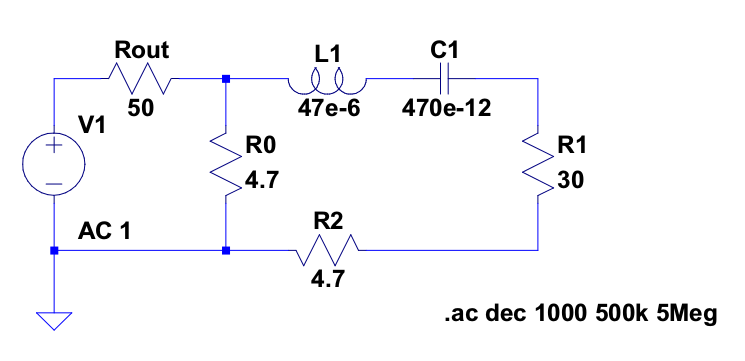
\includegraphics[width=8cm]{1AC.png}
  \caption{RLC直列回路(周波数特性の測定)}
\end{figure}

\subsubsection{周波数特性のシミュレート}
図1のように交流電圧源の電圧を\SI{1}{\volt}に設定し、周波数を\SI{500}{\kilo\hertz}から\SI{5}{\mega\hertz}まで、周波数が10倍になる間に1000回の割合で計算を行う。

\subsubsection{ステップ応答のシミュレート}
図2のように矩形波電圧源の電圧を\SI{1}{\volt}、立ち上がり時刻を\SI{0}{\second}、立ち上がり時間と立ち下がり時間を$10^{-50}\si{\second}$、立ち上がっている時間を\SI{1}{\second}、矩形波の周期を\SI{2}{\second}に設定し、時刻\SI{00}{\second}から\SI{5}{\micro\second}まで、\SI{50}{\pico\second}に一回計算を行う。
\begin{figure}[H]
  \centering
  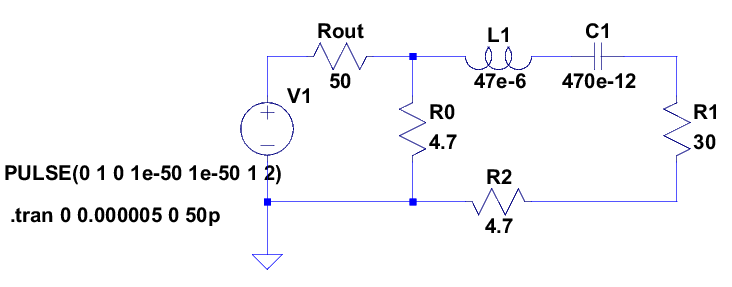
\includegraphics[width=8cm]{1step.png}
  \caption{RLC直列回路(ステップ応答の測定)}
\end{figure}

\subsubsection{数値データのエクスポート}
LTSpiceI\hspace{-.1em}Vでは、回路を構成してシミュレート条件を指定して実行した後、file $\to$ exportで数値データを.txt形式で保存できる。

但し、完全なcsvファイルではないため、テキストエディタの全置換機能などで適宜プロットソフトが読みやすい形式にしてやる必要がある。
また、位相差は$[-180(^\circ): 180(^\circ)]$の範囲で数値データ化されてしまうため、グラフ化した際には値が一気に飛ぶように見えることもある。

\subsubsection{数値データのプロット}
数値データのプロットにはgnuplotを用いる。
CUIを用いて軸の範囲の設定や軸の目盛りの設定、グラフの出力形式などを設定できるが、スクリプトにすることも可能である。
以下、本実験での設定を掲載する。
\clearpage

\lstinputlisting[caption=gnuplotの設定内容(振幅特性の出力)]{1AC_I.plt}

\lstinputlisting[caption=gnuplotの設定内容(位相特性の出力)]{1AC_arg.plt}

\lstinputlisting[caption=gnuplotの設定内容(ステップ応答の出力)]{1step.plt}

\subsection{3次の0-R型フィルタの設計と伝達特性のシミュレート}
ButterworthフィルタとChebyshevフィルタとでは、設計段階の最初の規格化低域通過フィルタの設計のみ、手順が異なる。

最初に、図3に示す3次規格化低域通過フィルタの伝送関数は、
\begin{equation}
T(s) = 1/F(s) = L_1L_2C s^3 + L_1 s^2 + \left( L_1+L_2\right) s + 1
\end{equation}
である。
\begin{figure}
\centering
\begin{circuitikz}
\draw (6,1) to[short,-o] (8,1) to[short, o-](9,1) to [L, l=$L_{1}$] (9.5,1) to
 [short, -*] (10.5,1) to [short, *-] (11.5,1) to [L, l=$L_{2}$] (12,1) to [short, -o] (13,1) to[short, o-] (14,1);
\draw (10.5,1) to [C, l=$C$] (10.5,-1) ;
\draw (6,-1) to[short,-o] (8,-1) to[short, o-] (9,-1) to
 [short, -*] (10.5,-1) to [short, *-] (11.5,-1)  to [short, -o] (13,-1) ;
\draw (8,1) to [open, v=$V_{in}$] (8,-1);
\draw (13,1) to [open, v=$V_{out}$] (13,-1) to[short, o-] (14,-1);
\draw (6,1) to[vsourcesin, l=$V_s$] (6,-1);
\draw (14,1) to[R, l=$\SI{1}{\ohm}$] (14,-1);
\end{circuitikz}
\caption{3次規格化低域通過フィルタ}
\end{figure}

\subsubsection{3次Butterworth規格化低域通過フィルタの設計}
3次Butterworth規格化低域通過フィルタの伝送関数は、
\begin{equation}
T(s)  = s^3 + 2s^2 + 2s + 1
\end{equation}
これと式(6)との右辺同士を比較して、$L_1$、$L_2$、$C$の値を決めれば良い。

\subsubsection{3次Chebyshev規格化低域通過フィルタの設計}
Chebyshevフィルタにはリプルの程度を決める値である$\epsilon$があるが、これが1.0であるフィルタを設計する。
3次Chebyshev規格化低域通過フィルタの伝達関数を求めるために、2.3にある法で極を求める。
\begin{eqnarray}
a &=& (\pi/6)(2k+1) \hspace{4pt} {\rm for}\hspace{4pt} k = 1, 2, 3, 4, 5, 6  \\
b &=& \pm (1/3)\sinh^{-1}(1)\\
\end{eqnarray}
の下で、極は
\begin{equation}
s = \sin a \sinh b + j \cos a \cosh b
\end{equation}
で表される12個(うち半分は重複するので実質は6個)のうち、複素平面上左反面にある3つである。
この3つを数値的に求め、式(6)との比較を行って$L_1$、$L_2$、$C$の値を決めるpythonのコードを以下に示す。
\lstinputlisting[caption=極の数値解を求める]{Cheby.py}
これを実行した後、最終行に出力される結果を用いる。

\subsection{インピーダンススケーリングと周波数変換}
\subsubsection{低域通過フィルタ}
遮断周波数\SI{1.5}{\kilo\hertz}、出力側インピーダンス$R = 50[\si{\ohm}]$の
低域通過フィルタを設計する。
回路の要素の変換は表1に示した変数変換の下で、以下の通り行われる。

\begin{table}[htb]
  \begin{center}
    \caption{要素の置換}
    \begin{tabular}{|l||c|c|} \hline
       & インダクタンス & キャパシタンス\\ \hline \hline
      基準 & $L=L_o$ & $C=C_o$ \\
      変換後 & $L=L_oR/\omega_c$ & $C=C_o/\omega_cR$ \\ \hline
    \end{tabular}
    \\ 但し、$\omega_c$が遮断角周波数
  \end{center}
\end{table}

\subsubsection{高域通過フィルタ}
遮断周波数\SI{1.5}{\kilo\hertz}、出力側インピーダンス$R = 50[\si{\ohm}]$の
低域通過フィルタを設計する。
回路の要素の変換は表1に示した変数変換の下で、以下の通り行われる。

\begin{table}[htb]
  \begin{center}
    \caption{要素の置換}
    \begin{tabular}{|l||c|c|} \hline
       & インダクタンス & キャパシタンス\\ \hline \hline
      基準 & $L=L_o$ & $C=C_o$ \\
      変換後 & $C=1/L_oR\omega_c$ & $L=R/C_o\omega_c$ \\ \hline
    \end{tabular}
    \\ 但し、$\omega_c$が遮断角周波数
  \end{center}
\end{table}

\subsubsection{帯域通過フィルタ}
中心周波数\SI{1.5}{\kilo\hertz}、出力側インピーダンス$R = 50[\si{\ohm}]$の
帯域通過フィルタを設計する。
帯域幅はButterworthフィルタが\SI{1}{\kilo\hertz}、Chebyshevフィルタが\SI{500}{\hertz}である。

回路の要素の変換は表1に示した変数変換の下で、以下の通り行われる。

\begin{table}[htb]
  \begin{center}
    \caption{要素の置換}
    \begin{tabular}{|l||c|c|} \hline
       & インダクタンス & キャパシタンス\\ \hline \hline
      基準 & $L=L_o$ & $C=C_o$ \\
      変換後 & $L=L_o/R\omega_b$と$C=\omega_b/L_o\omega_0^2R$の直列 & $L=\omega_bR/\omega_0^2C_o$ と $C=C_o/\omega_bR$の並列 \\ \hline
    \end{tabular}
    \\ 但し、$\omega_0$が中心角周波数、$\omega_b$が帯域幅
  \end{center}
\end{table}

\subsection{伝達特性のシミュレート}
\subsubsection{周波数応答のシミュレート}
振幅特性及び周波数特性のシミュレートは、\SI{1}{\volt}の正弦波に対する応答を見る。
それぞれのフィルタのシミュレート条件を表6にまとめる。

\begin{table}[htb]
  \begin{center}
    \caption{シミュレートの条件(周波数応答)}
    \begin{tabular}{|l||c|c|c|} \hline
      フィルタ & 周波数下限[\si{\hertz}] & 周波数上限[\si{\hertz}] & 計算頻度$^*$\\ \hline \hline
      LPF & 100 & 5000 & 10000\\
      ButterwothHPF & 100 & 5000 & 10000 \\ 
      ChebyshevHPF & 1000 & 30000 & 10000 \\ 
      ButterwothBPF & 1000 & 22000 & 10000 \\ 
      ChebyshevBPF & 100 & 10000 & 10000 \\ 
      \hline
    \end{tabular}
    \\ $^*$周波数が10倍になる間に何回計算を行うか
  \end{center}
\end{table}

\subsubsection{ステップ応答のシミュレート}
ステップ応答のシミュレートは、\SI{1}{\volt}の方形波に対する、\SI{0.01}{\second}までの応答を見る。電源の設定を表7にまとめる。

\begin{table}[htb]
  \begin{center}
    \caption{ステップ応答解析における電源の設定}
    \begin{tabular}{|l||c|} \hline
      立ち上がり前電圧 & \SI{0}{\volt} \\ 
      立ち上がり後電圧 & \SI{1}{\volt} \\
      立ち上がり時刻 & \SI{0}{\second} \\ 
      立ち上がり時間 & $10^{50}$\si{\second} \\ 
      立ち下がり時間 & $10^{50}$\si{\second} \\ 
      立ち上がり持続時間 & \SI{1}{\second} \\
      周期  & \SI{2}{\second} \\
      \hline
    \end{tabular}
  \end{center}
\end{table}

\section{使用器具}

\subsection{回路シミュレータ}
\begin{description}
\item[シミュレータ] LTSpiceI\hspace{-.1em}V ver.4.23
\end{description}

\subsection{シミュレータ実行環境}
\begin{description}
\item[PC] Dell Latitude E6430
\item[OS] Windows 10 Education
\item[CPU] Intel(R) Core(TM) i7-3630QM CPU @ 2.40GHz
\item[メモリ] 16GB
\end{description}

\subsection{プロットソフト}
\begin{description}
\item[プロットソフト] gnuplot 4.6 patchlevel 4
\end{description}
\subsection{プロットソフト実行環境}
\begin{description}
\item[OS] Ubuntu14.04LTS
\end{description}
その他はシミュレータ実行環境に同じ。

\section{実験結果}

\subsection{回路シミュレータLTSpiceI\hspace{-.1em}Vでの簡単な回路のシミュレートとその数値データのプロット}
プロット結果はそれぞれ図4,5,6の通りであった。

\begin{figure}[H]
  \centering
  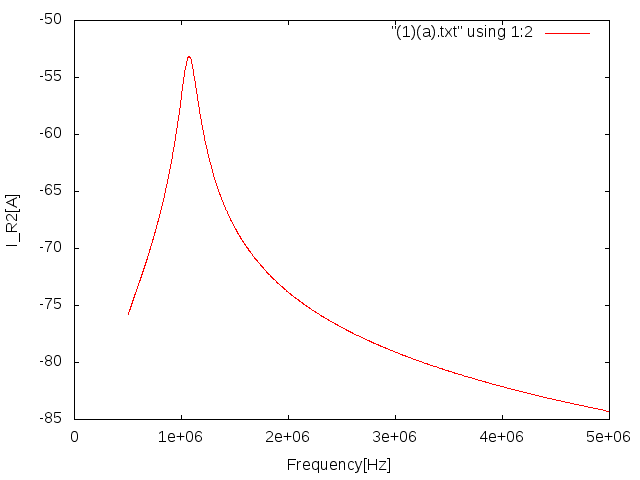
\includegraphics[width=8cm]{1AC_Igraf.png}
  \caption{RLC直列回路の周波数による振幅特性}
\end{figure}

\begin{figure}[H]
  \centering
  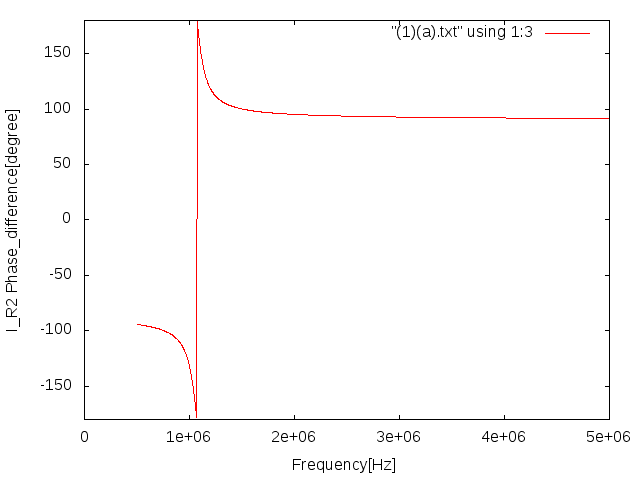
\includegraphics[width=8cm]{1AC_Agraf.png}
  \caption{RLC直列回路の周波数による位相特性}
\end{figure}

\begin{figure}[H]
  \centering
  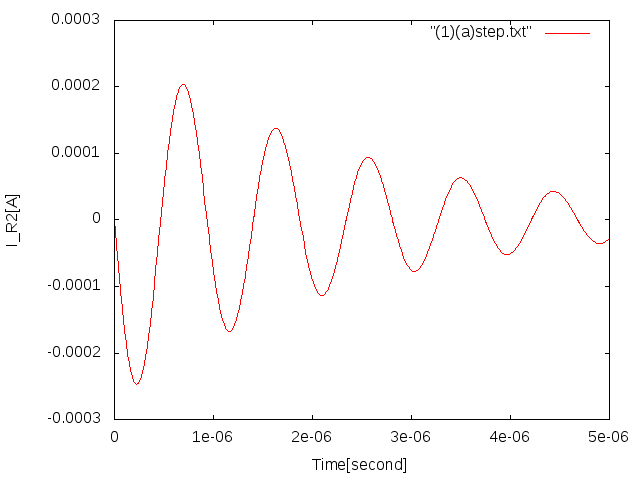
\includegraphics[width=8cm]{1stepgraf.png}
  \caption{RLC直列回路のステップ応答}
\end{figure}

\subsection{Butterworthフィルタ}
\subsubsection{規格化低域通過フィルタの設計}
設計の結果、
\begin{eqnarray}
L_1 &=& 1.5 \\
L_2 &=& 0.5 \\
C &=& 4/3 \simeq 1.333
\end{eqnarray}
となった。この数値を基準として、以後の各種フィルタの設計を行った。

\subsubsection{低域通過フィルタ}
遮断周波数\SI{1.5}{\kilo\hertz}のButterworth低域通過フィルタは、図7(図中のuは\si{\micro}である。以下同じ。)に示す通りとなった。そのシミュレート結果も、図8〜10に示す。

\begin{figure}[H]
    \begin{tabular}{cc}
      %---- 最初の図 ---------------------------
      \begin{minipage}[t]{0.45\hsize}
        \centering
        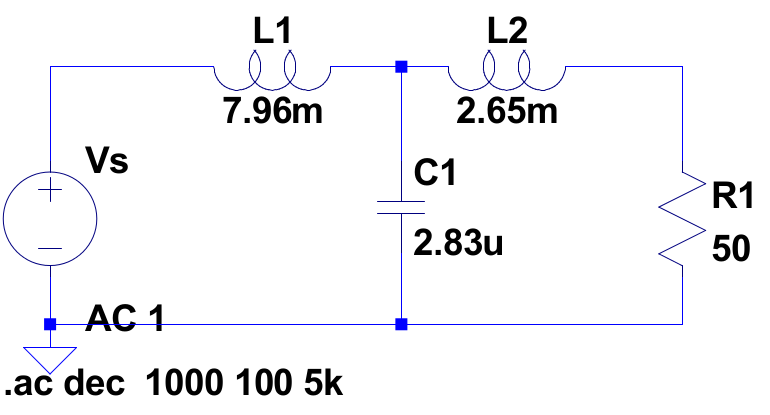
\includegraphics[width=8cm]{ButLPF.png}
        \caption{ButterworthLPF($f_c = 1500$)}
      \end{minipage} &
      %---- 2番目の図 --------------------------
      \begin{minipage}[t]{0.45\hsize}
        \centering
        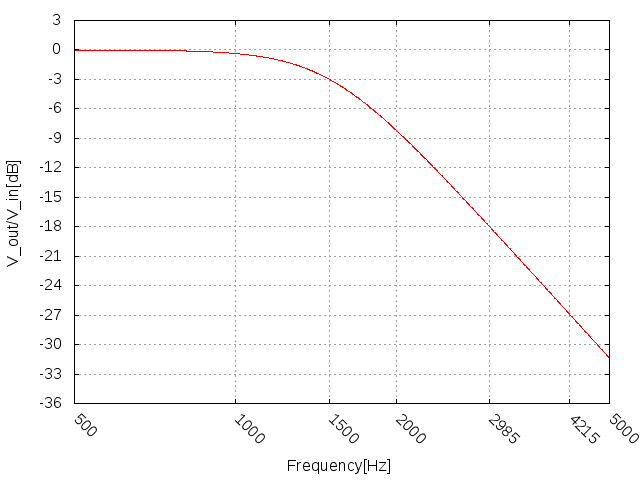
\includegraphics[width = 8cm]{BLPF_Vgraf.png}
        \caption{ButterworthLPFの振幅特性}
      \end{minipage}
      %---- 図はここまで ----------------------
    \end{tabular}
  \end{figure}
  \begin{figure}[H]
      \begin{tabular}{cc}
        %---- 最初の図 ---------------------------
        \begin{minipage}[t]{0.45\hsize}
          \centering
          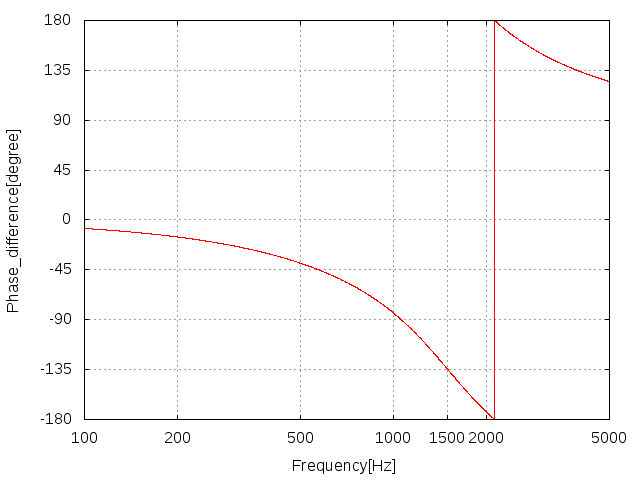
\includegraphics[width=8cm]{BLPF_Agraf.png}
          \caption{ButterworthLPFの位相特性}
        \end{minipage} &
        %---- 2番目の図 --------------------------
        \begin{minipage}[t]{0.45\hsize}
          \centering
          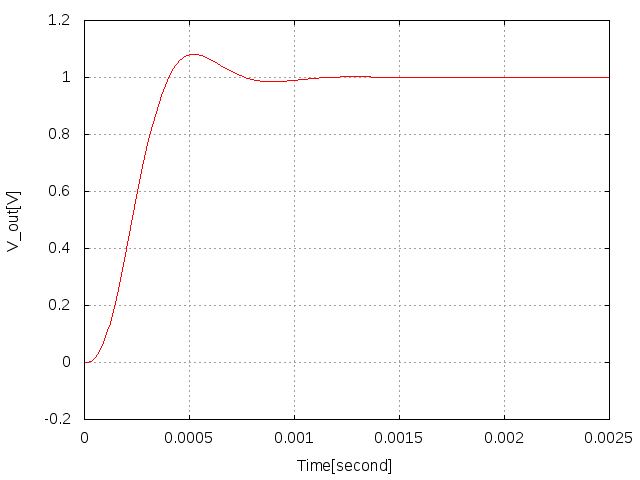
\includegraphics[width = 8cm]{BLPFstep.png}
          \caption{ButterworthLPFのステップ応答}
        \end{minipage}
        %---- 図はここまで ----------------------
      \end{tabular}
    \end{figure}
 
 \subsubsection{高域通過フィルタ}
 遮断周波数\SI{1.5}{\kilo\hertz}のButterworth高域通過フィルタは、図11に示す通りとなった。そのシミュレート結果も、図12〜14に示す。
 
 \begin{figure}[H]
     \begin{tabular}{cc}
       %---- 最初の図 ---------------------------
       \begin{minipage}[t]{0.45\hsize}
         \centering
         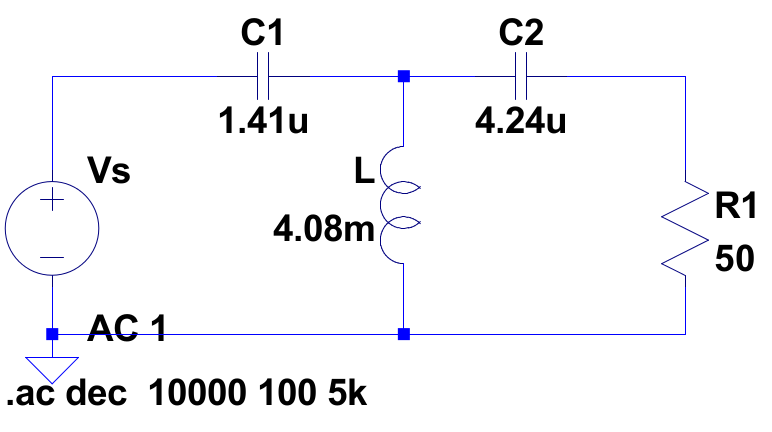
\includegraphics[width=8cm]{ButHPF.png}
         \caption{ButterworthHPF($f_c = 1500$)}
       \end{minipage} &
       %---- 2番目の図 --------------------------
       \begin{minipage}[t]{0.45\hsize}
         \centering
         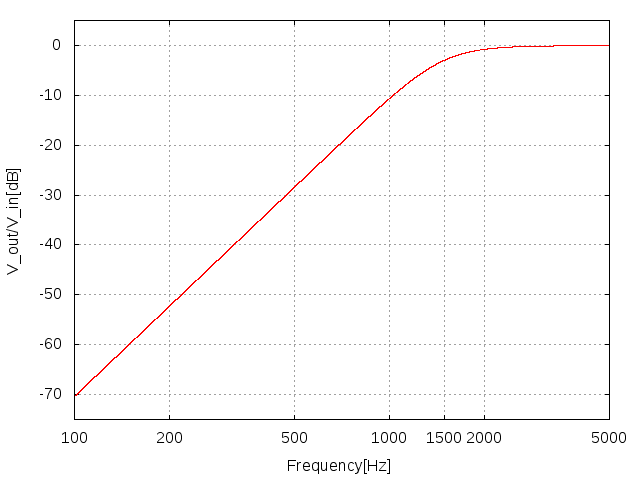
\includegraphics[width = 8cm]{BHPF_Vgraf.png}
         \caption{ButterworthHPFの振幅特性}
       \end{minipage}
       %---- 図はここまで ----------------------
     \end{tabular}
   \end{figure}
   \begin{figure}[H]
       \begin{tabular}{cc}
         %---- 最初の図 ---------------------------
         \begin{minipage}[t]{0.45\hsize}
           \centering
           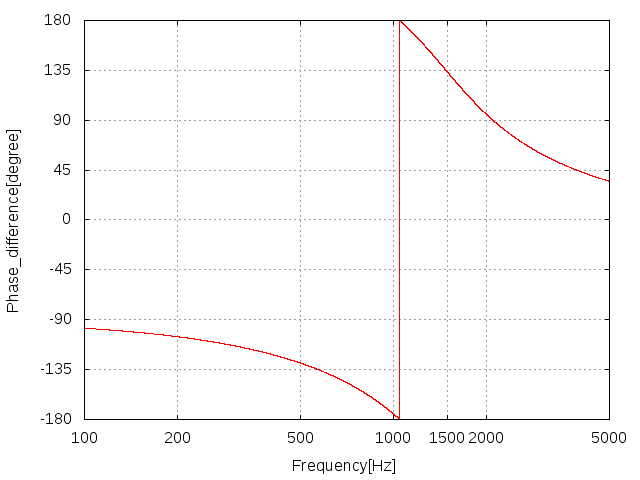
\includegraphics[width=8cm]{BHPF_Agraf.png}
           \caption{ButterworthHPFの位相特性}
         \end{minipage} &
         %---- 2番目の図 --------------------------
         \begin{minipage}[t]{0.45\hsize}
           \centering
           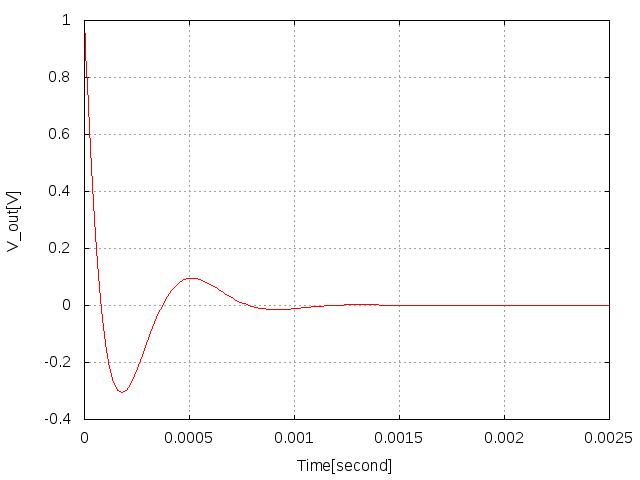
\includegraphics[width = 8cm]{BHPFstep.png}
           \caption{ButterworthHPFのステップ応答}
         \end{minipage}
         %---- 図はここまで ----------------------
       \end{tabular}
     \end{figure}

 \subsubsection{帯域通過フィルタ}
 中心周波数\SI{1.5}{\kilo\hertz}、帯域幅\SI{1}{\kilo\hertz}のButterworth帯域通過フィルタは、図15に示す通りとなった。そのシミュレート結果も、図16〜18に示す。
 
 \begin{figure}[H]
     \begin{tabular}{cc}
       %---- 最初の図 ---------------------------
       \begin{minipage}[t]{0.45\hsize}
         \centering
         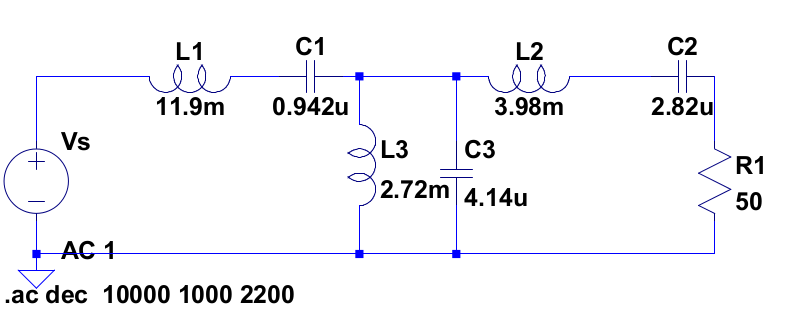
\includegraphics[width=8cm]{ButBPF.png}
         \caption{ButterworthBPF($f_0 = 1500$)}
       \end{minipage} &
       %---- 2番目の図 --------------------------
       \begin{minipage}[t]{0.45\hsize}
         \centering
         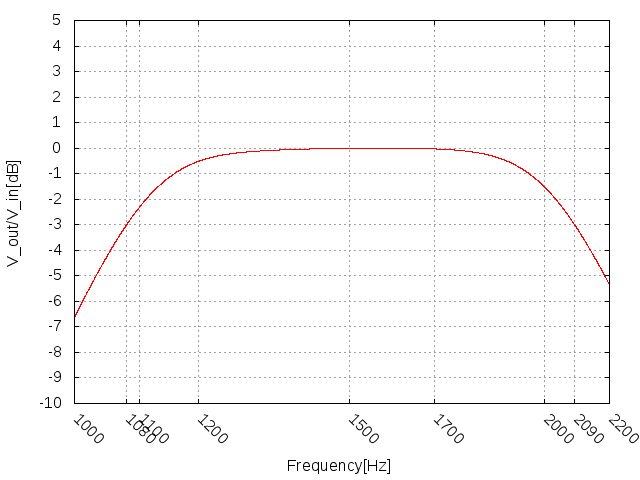
\includegraphics[width = 8cm]{BBPF_Vgraf.png}
         \caption{ButterworthBPFの振幅特性}
       \end{minipage}
       %---- 図はここまで ----------------------
     \end{tabular}
   \end{figure}
   \begin{figure}[H]
       \begin{tabular}{cc}
         %---- 最初の図 ---------------------------
         \begin{minipage}[t]{0.45\hsize}
           \centering
           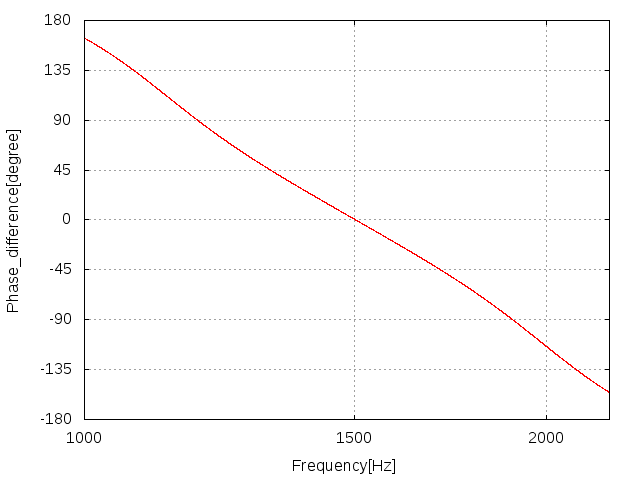
\includegraphics[width=8cm]{BBPF_Agraf.png}
           \caption{ButterworthBPFの位相特性}
         \end{minipage} &
         %---- 2番目の図 --------------------------
         \begin{minipage}[t]{0.45\hsize}
           \centering
           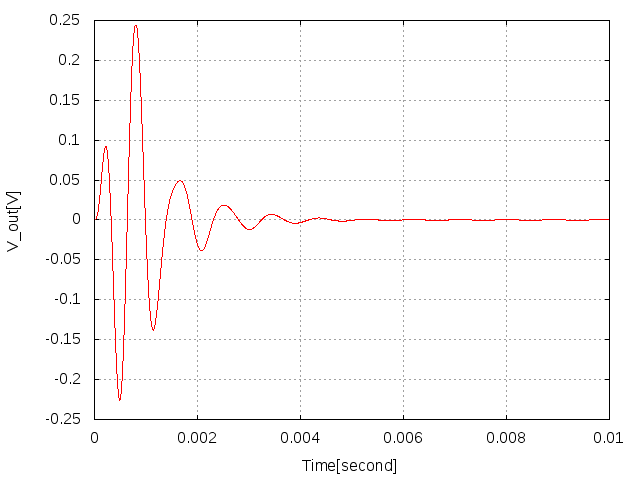
\includegraphics[width = 8cm]{BBPFstep.png}
           \caption{ButterworthBPFのステップ応答}
         \end{minipage}
         %---- 図はここまで ----------------------
       \end{tabular}
     \end{figure}
          
\subsection{Chebyshevフィルタ}
\subsubsection{規格化低域通過フィルタの設計}
設計の結果、
\begin{eqnarray}
L_1 &=& 2.033 \\
L_2 &=& 1.678 \\
C &=& 1.173
\end{eqnarray}
となった。この数値を基準として、以後の各種フィルタの設計を行った。

\subsubsection{低域通過フィルタ}
遮断周波数\SI{1.5}{\kilo\hertz}のChebyshev低域通過フィルタは、図19に示す通りとなった。そのシミュレート結果も、図20〜22に示す。

\begin{figure}[H]
    \begin{tabular}{cc}
      %---- 最初の図 ---------------------------
      \begin{minipage}[t]{0.45\hsize}
        \centering
        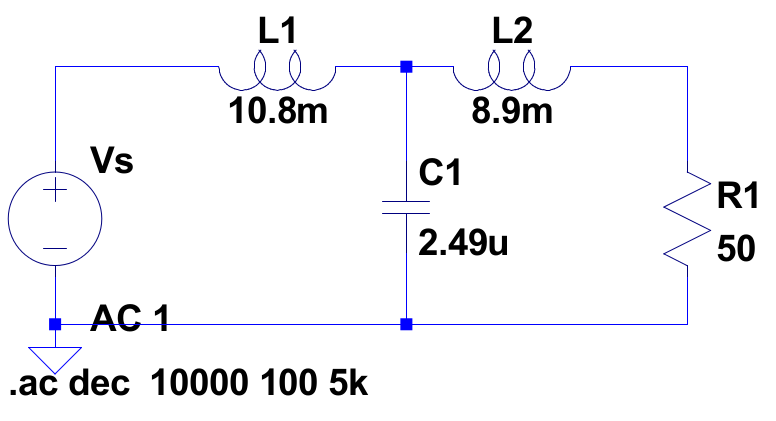
\includegraphics[width=8cm]{CheLPF.png}
        \caption{ChebyshevLPF($f_c = 1500$)}
      \end{minipage} &
      %---- 2番目の図 --------------------------
      \begin{minipage}[t]{0.45\hsize}
        \centering
        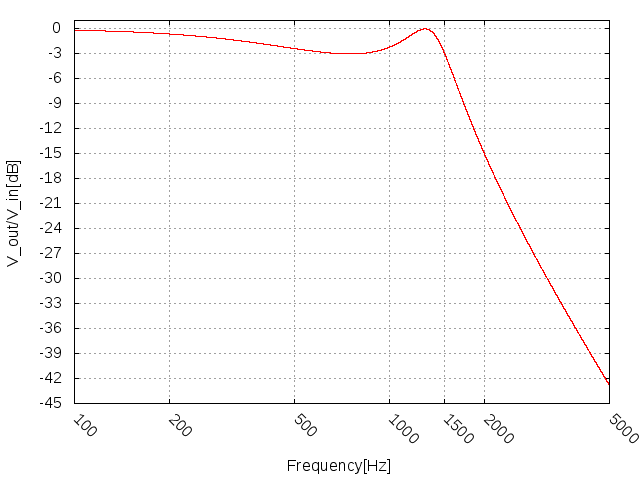
\includegraphics[width = 8cm]{CLPF_Vgraf.png}
        \caption{ChebyshevLPFの振幅特性}
      \end{minipage}
      %---- 図はここまで ----------------------
    \end{tabular}
  \end{figure}
  \begin{figure}[H]
      \begin{tabular}{cc}
        %---- 最初の図 ---------------------------
        \begin{minipage}[t]{0.45\hsize}
          \centering
          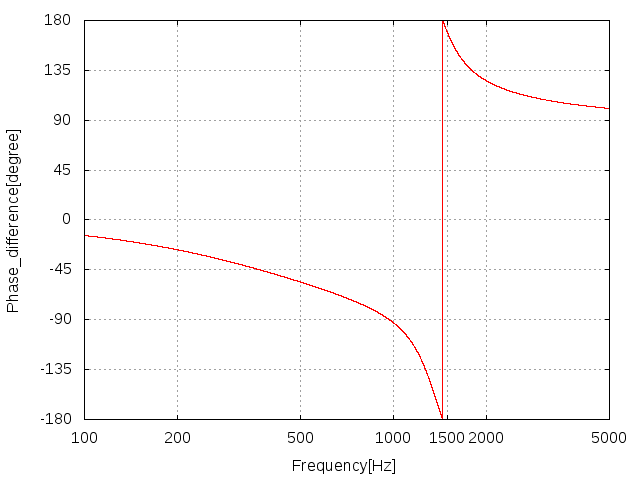
\includegraphics[width=8cm]{CLPF_Agraf.png}
          \caption{ChebyshevLPFの位相特性}
        \end{minipage} &
        %---- 2番目の図 --------------------------
        \begin{minipage}[t]{0.45\hsize}
          \centering
          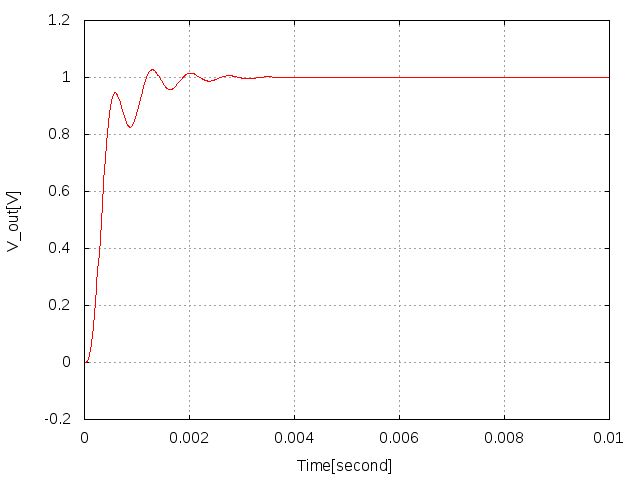
\includegraphics[width = 8cm]{CLPFstep.png}
          \caption{ChebyshevPFのステップ応答}
        \end{minipage}
        %---- 図はここまで ----------------------
      \end{tabular}
    \end{figure}
 
 \subsubsection{高域通過フィルタ}
 遮断周波数\SI{1.5}{\kilo\hertz}のChebyshev高域通過フィルタは、図23に示す通りとなった。そのシミュレート結果も、図24〜26に示す。
 
 \begin{figure}[H]
     \begin{tabular}{cc}
       %---- 最初の図 ---------------------------
       \begin{minipage}[t]{0.45\hsize}
         \centering
         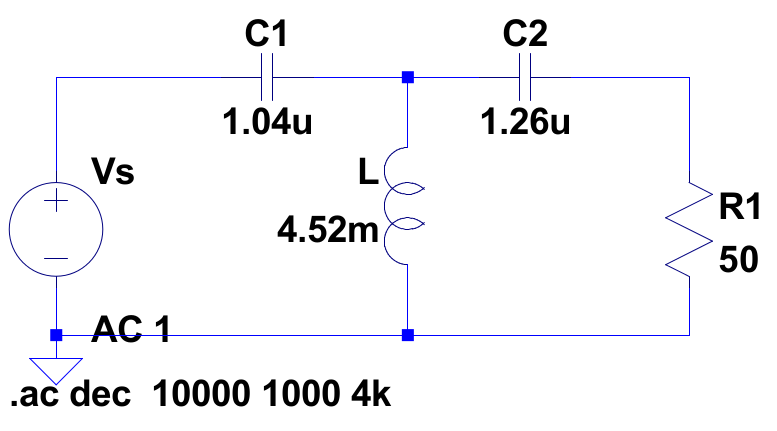
\includegraphics[width=8cm]{CheHPF.png}
         \caption{ChebyshevHPF($f_c = 1500$)}
       \end{minipage} &
       %---- 2番目の図 --------------------------
       \begin{minipage}[t]{0.45\hsize}
         \centering
         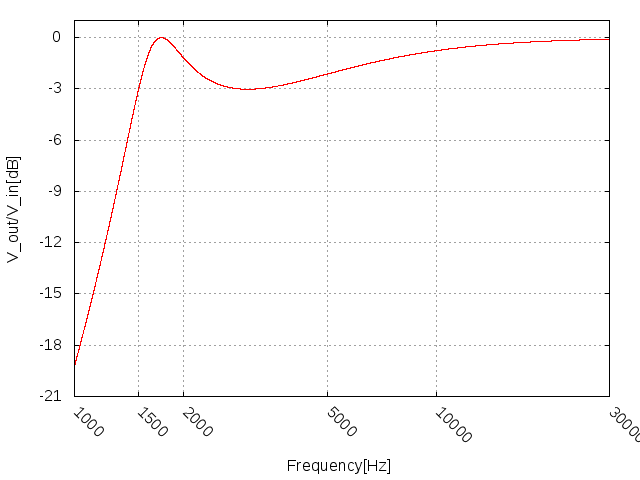
\includegraphics[width = 8cm]{CHPF_Vgraf.png}
         \caption{ChebyshevHPFの振幅特性}
       \end{minipage}
       %---- 図はここまで ----------------------
     \end{tabular}
   \end{figure}
   \begin{figure}[H]
       \begin{tabular}{cc}
         %---- 最初の図 ---------------------------
         \begin{minipage}[t]{0.45\hsize}
           \centering
           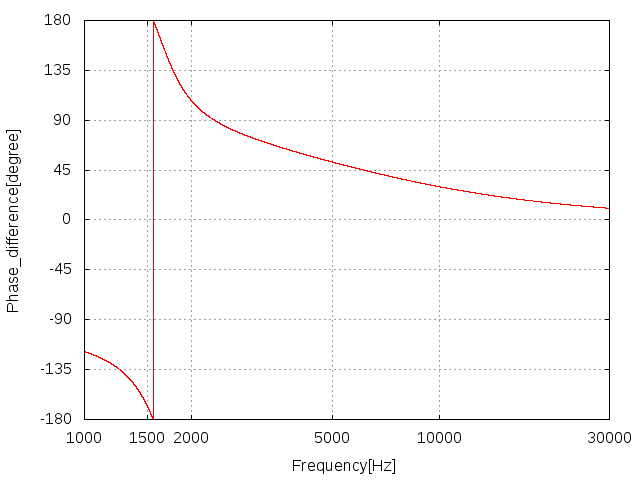
\includegraphics[width=8cm]{CHPF_Agraf.png}
           \caption{ChebyshevHPFの位相特性}
         \end{minipage} &
         %---- 2番目の図 --------------------------
         \begin{minipage}[t]{0.45\hsize}
           \centering
           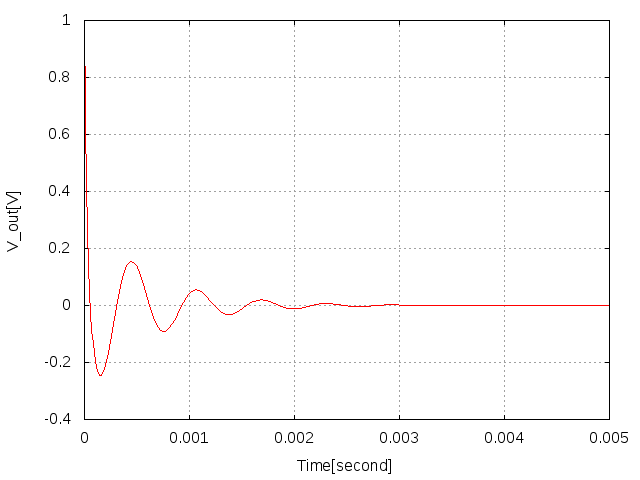
\includegraphics[width = 8cm]{CHPFstep.png}
           \caption{ChebyshevHPFのステップ応答}
         \end{minipage}
         %---- 図はここまで ----------------------
       \end{tabular}
     \end{figure}

 \subsubsection{帯域通過フィルタ}
 中心周波数\SI{1.5}{\kilo\hertz}、帯域幅\SI{500}{\hertz}のChebyshev帯域通過フィルタは、図27に示す通りとなった。そのシミュレート結果も、図28〜30に示す。
 
 \begin{figure}[H]
     \begin{tabular}{cc}
       %---- 最初の図 ---------------------------
       \begin{minipage}[t]{0.45\hsize}
         \centering
         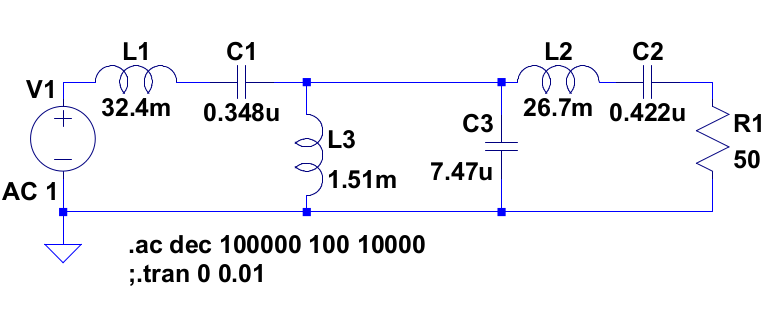
\includegraphics[width=8cm]{CheBPF.png}
         \caption{ChebyshevBPF($f_0 = 1500$)}
       \end{minipage} &
       %---- 2番目の図 --------------------------
       \begin{minipage}[t]{0.45\hsize}
         \centering
         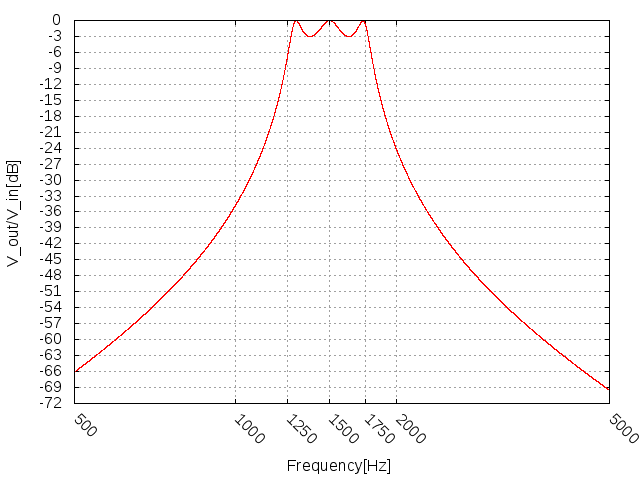
\includegraphics[width = 8cm]{CBPF_Vgraf.png}
         \caption{ChebyshevBPFの振幅特性}
       \end{minipage}
       %---- 図はここまで ----------------------
     \end{tabular}
   \end{figure}
   \begin{figure}[H]
       \begin{tabular}{cc}
         %---- 最初の図 ---------------------------
         \begin{minipage}[t]{0.45\hsize}
           \centering
           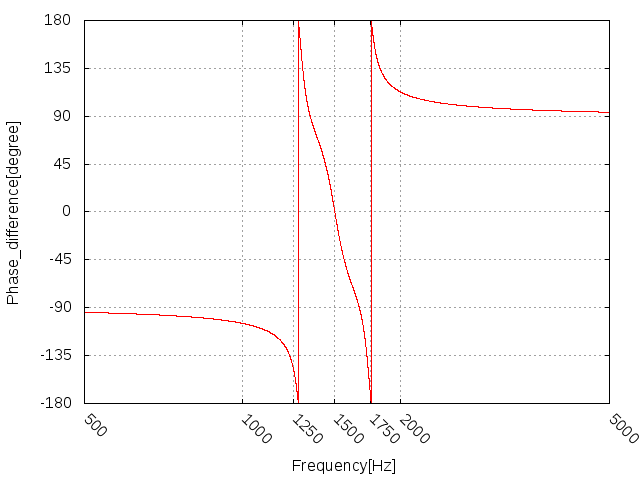
\includegraphics[width=8cm]{CBPF_Agraf.png}
           \caption{ChebyshevBPFの位相特性}
         \end{minipage} &
         %---- 2番目の図 --------------------------
         \begin{minipage}[t]{0.45\hsize}
           \centering
           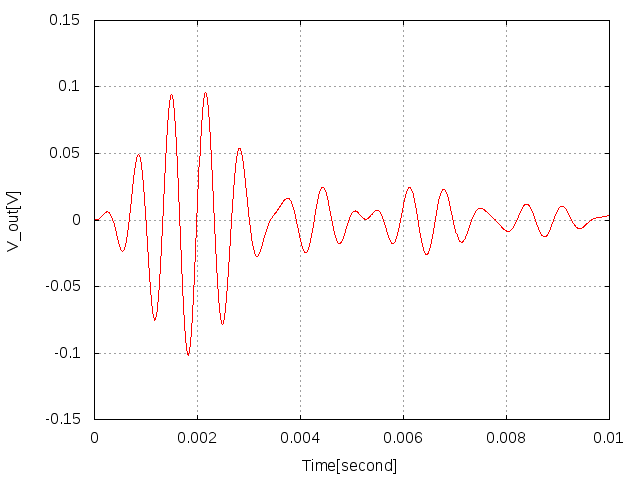
\includegraphics[width = 8cm]{CBPFstep.png}
           \caption{ChebyshevBPFのステップ応答}
         \end{minipage}
         %---- 図はここまで ----------------------
       \end{tabular}
     \end{figure}

\section{考察}
\subsection{3次低域通過フィルタの伝達特性}
3次フィルタとしての特徴は、主として振幅特性に現れている。
これは、Butterworth及びChebyshevフィルタが主たる設計思想として通過域と減衰域に注目していることが大きな原因の一つであろうと思われる。

Butterworthフィルタでは、遮断域にn次フィルタの特性が表れる。
図8を見ると、\SI{2985}{\hertz}から\SI{4215}{\hertz}まででおおよそ\SI{-9}{\decibel}の損失が見られる。
\begin{equation}
\frac{-9}{\log_{10}4215 - \log_{10}2985} \simeq -60.059[\si{\decibel}]
\end{equation}
より、周波数の常用対数が1増加する間に$20\bullet3 = 60$\si{\decibel}の損失が発生するという理論値とほぼ等しい。

一方無極形通過域Chebyshevフィルタでは、次数が最も顕著に表れるのは通過域でのリプルの回数である。
n次の低域通過フィルタでは、少なくともn/2回のリプルが発生する。
図20を見れば、2回のリプルが発生していることがわかる。
(或いは、BPFのリプルの回数を数えるのが妥当だろう[次節参照]。)

\subsection{3次高域通過及び帯域通過フィルタの周波数特性}
高域通過フィルタについては、前節にて述べた低域通過フィルタと大きく変わらない。
Butterworthフィルタは遮断域での傾きが\SI{60}{\decibel}/decadeに、Chebyshevフィルタでは通過域で2回のリプルが発生している。

一方の帯域通過フィルタだが、振幅特性が左右対称なフィルタであるだけに、Chebyshevフィルタでは、リプルの数と次数の関係をより明確に読み取ることが出来る。
図28では通過域に明らかに3つの山が立っている。

\subsection{Butterworth帯域通過フィルタでの誤差}
図16を見ると、\SI{-3}{\decibel}を取る周波数は、およそ\SI{1080}{\hertz}と\SI{2090}{\hertz}で、その中心も\SI{1585}{\hertz}と、理論値から6%弱の誤差が出ている。
これは、周波数変換を行う際に電卓を用いて、幾らか数値を丸めているためであろうと考えられる。
数値を有効数字三桁に丸めながら演算を行ったので、相対的な丸め誤差の最小単位は、$ u = 1/2\bullet10^{-2}$である。
構成要素の置き換えの計算だけでも二項演算子を4回使うから、その誤差は$\sqrt{4}u = 10^{-2}$程度発生する。
そこから更に周波数と振幅の関係に記述しなおされると、ひと桁台%の誤差は妥当なように思われる。

\section{参考資料}
\begin{enumerate}
\item 東京大学工学部 電子情報工学科・電気電子工学科(2016)『電気電子情報第一(前期)実験 テキスト』
\item R.M.Fano \& A.W.Lawson (1948) 菅原英彦訳(2009) 『マイクロ波フィルタの理論』丸善プラネット
\item 古賀利郎(1978)『伝送回路』コロナ社
\item 幸谷智紀(2005)『数値計算における誤差について –数値微分を例に–』http://na-inet.jp/na/na\_error\_diff.pdf

\end{enumerate}


\end{document}
